
% %NOTE:
% % CHECKED WITH SLIDES: YES!
% % CHECKED WITH EXERCISES: NO -- TODO
% % MISSING: -

\section{Low Power Design}

\subsection{General}
Performance-Power Efficiency list (Operations/Watt). From bad (low) to good (high performance while using low energy).
\begin{enumerate}[noitemsep]
\item General-purpose processors
\item Application-specific instruction set processors (ASIPs) 
\item Programmable hardware: FPGA
\item Application-specific integrated circuits (ASICs)
\end{enumerate}

\subsection{Power and Energy}
\begin{theorem}[Energy]
$E = \int P(t) dt$. To save energy, we can decrease the execution time or use less power.
\end{theorem}

\subsubsection{Low power consumption}
Important for: 
\begin{itemize}[noitemsep]
\item the design of the power supply
\item the design of voltage regulators
\item the dimensioning of interconnect
\item cooling
\end{itemize}

\subsubsection{Low energy consumption}
Important due to 
\begin{itemize}[noitemsep]
\item restricted availability of energy
\item limited battery capacities
\item high costs of energy
\item long term: low temperatures
\end{itemize}

\subsubsection{Power Consumption of CMOS Gate}
\begin{itemize}[noitemsep]
\item leakage current: caused by electronic devices attached to the capacitors, such as transistors or diodes, which conduct a small amount of current even when they are turned off
\item short circuit current: For a short time, both are conducting.
\item switching current: Current used for switching the gate
\end{itemize}

\begin{tnote}
Without switching, there is no short circuiting current and no switching current!
\end{tnote}

\subsubsection{Types of Power Consumption/ Consumption of CMOS Processors}
\begin{itemize}[noitemsep]
\item Dynamic power consumption: charging and discharging capacitors
\item Short circuit power consumption due to switching
\item Leakage: diodes, translators. The smaller the technology, the more important the leakage current
\end{itemize}



\subsubsection{Dynamic Voltage Scaling - DVS}

\begin{definition} [Supply Voltage]
$V_{dd}$
\end{definition}

\begin{definition} [Switching activity]
$\alpha$
\end{definition}

\begin{definition} [Load Capacity]
$C_L$
\end{definition}

\begin{definition} [Clock frequency]
$f$
\end{definition}

\begin{definition} [threshold voltage]
$V_T$ where $V_T \ll V_{dd}$
\end{definition}

\begin{theorem}[Power consumption of CMOS
circuits (ignoring leakage)] 
${ P \sim \alpha C_L V^2_{dd} f }$
\end{theorem}

\begin{theorem}[Delay for CMOS circuits] 
${ \tau \sim C_L \frac{V_{dd}}{(V_{dd} - V_T)^2} \approx C_L \frac{1}{V_{dd}}}$ with $V_T \ll V_{dd}$
\end{theorem}


\begin{itemize}[noitemsep]
\item Decreasing $V_{dd}$ reduces $P$ quadratically ($f$ constant)
\item The gate delay increases reciprocally with decreasing $V_{dd}$
\item Maximal frequency $f_{max}$ decreases linearly with decreasing $V_{dd}$
\item Assuming $\alpha, C_L$ constant, then $P \sim V_{dd}^3$
\end{itemize}

\begin{theorem}[Energy]
$E \sim \alpha C_L V^2_{dd} f t = \alpha C_L V^2_{dd} * (\#cycles) $
\end{theorem}

\begin{itemize}[noitemsep]
\item Reduce the supply voltage $V_{dd}$
\item Reduce switching activity $\alpha$
\item Reduce the load capacitance $C_L$
\item Reduce the number of cycles $\#cycles$
\end{itemize}


\subsubsection{Power Supply Gating}
Power gating is one of the most effective ways of minimizing static power consumption (leakage). Cut-off power supply to inactive units/components


\subsection{Parallelism}
A given task with $V_{dd}$ and $f_{max}$ which uses $E_1$ energy is split to two units with $V_{dd}/2$ and $f_{max}/2$. Both work in parallel. This results in a quarter of the energy used before: $E_2 = \frac{1}{4}E_1$. Calculated by inserting in the formulas.

\subsection{Pipelining}
A given task with $V_{dd}$ and $f_{max}$ which uses $E_1$ energy is split to two units with $V_{dd}/2$ and $f_{max}/2$. The units are in series, so the first does a pre-processing and the second unit finishes the task. This results in a quarter of the energy used before: $E_2 = \frac{1}{4}E_1$. Calculated by inserting in the formulas.


\subsection{VLIW}
Use the degree of parallelism to develop a chip with many computational units, (deeply) pipelined to make use of Parallelism and Pipelining to save energy. Explicit parallelism by a parallel instruction set or parallelization is done offline (compiler). Problem is that chip takes now different code: needs a chip on the chip which does the translation or re-compile the code or use a software compiler at run time to translate the instructions.

\subsection{Dynamic Voltage Scaling}
We know that: a) Not all components require same performance. and b) Required performance may change over time. Make now use of these two facts


\begin{theorem}[DVS]
If the power-consumption is a convex function of the supply voltage, running at a constant frequency (voltage) minimizes the energy consumption for dynamic voltage scaling.
\end{theorem}

\subsection{YDS Algorithm for Offline Scheduling}
Solves the problem of scheduling tasks such that all these tasks can be finished no later than their deadlines and the energy consumption is  minimized.

\begin{definition}[Intensity]
Intensity $G([z, z'])$ in some time interval $[z, z']$: average accumulated execution time of all tasks that have arrival and deadline in $[z, z']$ relative to the length of the interval $z'-z$.\\
$V'([z, z']) = \{ v_i \in V: z \leq a_i \le d_i \leq z' \} $\\
$ G([z, z'])  = \sum\limits_{v_i \in V'([z, z'])} c_i/(z'-z)$
\end{definition}


\begin{enumerate}
\item Execute jobs in the interval with the highest intensity by using the earliest-deadline first schedule and running at the intensity as the frequency.
\item Adjust the arrival times and deadlines by excluding the
possibility to execute at the previous critical intervals.
\item Run the algorithm for the revised input again.
\item Put pieces together. Run the tasks with EDF with the computed frequencies. Output is a diagram which shows at what time which threads is scheduled with what frequency.
\end{enumerate}

\begin{theorem}
The algorithm guarantees the minimal energy consumption while satisfying the timing constraints
\end{theorem}

\begin{theorem}
Time complexity is $O(N^3)$ where $N$ is the number of tasks in $V$. Number of iterations is at most $N$.
\end{theorem}

\begin{theorem}
For periodic real-time tasks with deadline=period, running at constant speed with 100\% utilization under EDF has minimum energy consumption while satisfying the timing constraints.
\end{theorem}

\subsection{DVS - Online Scheduling on One Processor}
Continuously update to the best schedule for all arrived tasks. Compute the intensity for each incoming task and update

\begin{theorem}
Compared to the optimal off-line solution, the on-line schedule uses at most 27 times of the minimal energy consumption.
\end{theorem}


\subsection{Dynamic Power Management (DPM)}


\begin{itemize}[noitemsep]
\item Shut down devices if they are not to be used
\item Wake them up when service is required
\item Can reduce leakage and dynamic pow
\item States:
	\begin{itemize}
		\item Run: operational
		\item Idle: a SW routine may stop the CPU when not in use, while monitoring interrupts
		\item Sleep: Shutdown of on-chip activity
	\end{itemize}
\end{itemize}

Problem: overhead due to shutdown and wakeup delay

\begin{definition}[DVS Critical frequency (voltage)]
DVS Critical frequency (voltage): running at any frequency/voltage lower than this frequency is not worthwhile for execution.
\end{definition}

\subsection{Procrastination Schedule}
Run the YDS algorithm but round all frequencies up to the critical frequency. If the frequency determined by the YDS algorithm is smaller than the critical frequency, there will be sleep time for the processor, since tasks are faster executed in that intervall than needed. To reduce the number of turn on/offs and maximize the sleep time, the tasks are bundled together and executed as late as possible.

\begin{figure}[ht]
	\centering
  	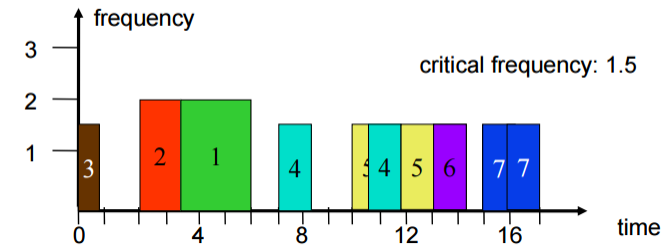
\includegraphics[scale=0.4]{img/9_yds_procrast.png}
	\caption{YDS with rounding up and procrastrination}
	\label{fig_yds_procrast}
\end{figure}


\cleardoublepage

